\documentclass[a4paper,11pt]{jsarticle}


% 数式
\usepackage{amsmath,amsfonts}
\usepackage{bm}
\usepackage{siunitx}
% 画像
\usepackage[dvipdfmx]{graphicx}
\usepackage{booktabs}


\begin{document}

\title{}
\author{}
\date{\today}


\section{図の回路において、AB間のインピーダンスが周波数と無関係になるときの$C$の値を求めなさい。なお、$C$以外の素子の値は既知であるとし、また、$\omega Cr \ll 1$とみなせるものとします。}
\begin{figure}[htbp]
  \centering
  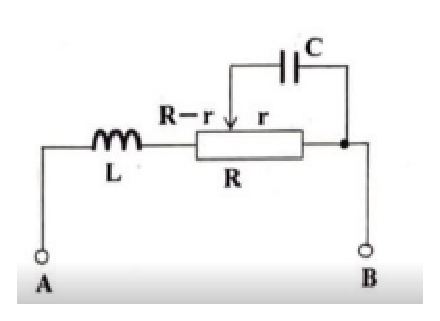
\includegraphics[width=7.5cm]{fig4.eps}
  \caption{}\label{fig1}
\end{figure}

AB間のインピーダンス$\dot{Z}$は、
\begin{align}
  \begin{split}
    \dot{Z}
    &=j\omega L +R-r+\frac{\frac{R}{j\omega C}}{r+\frac{1}{j\omega C}}\\
    &=j\omega L +R-r+\frac{r}{1+j\omega Cr}\\
    &=R-r+j\omega L+\frac{r(1-j\omega Cr)}{1+{(\omega Cr)}^{2}}
    \label{eq1}
  \end{split}
\end{align}
$\omega Cr \ll 1$より、
\begin{align}
  \begin{split}
    \dot{Z}\simeq R-r+j\omega L+r(1-j\omega Cr)
    &=R+j\omega (L-Cr^{2})
    \label{eq2}
  \end{split}
\end{align}
周波数と無関係であるとき、式\eqref{eq2}における虚部は0となるため、
\begin{align}
  \begin{split}
    L-Cr^{2}
    &=0\\
    C
    &=\frac{L}{r^{2}}
    \label{eq3}
  \end{split}
\end{align}
となる。

\end{document}